\documentclass[12pt]{article}
\usepackage{tikz} 
\usetikzlibrary{shapes}
\usetikzlibrary{arrows}
\usetikzlibrary{positioning}
\usetikzlibrary{patterns}
\usetikzlibrary{calc}


\usepackage{xepersian}
\settextfont[Scale=1]{Vazir}

\begin{document}



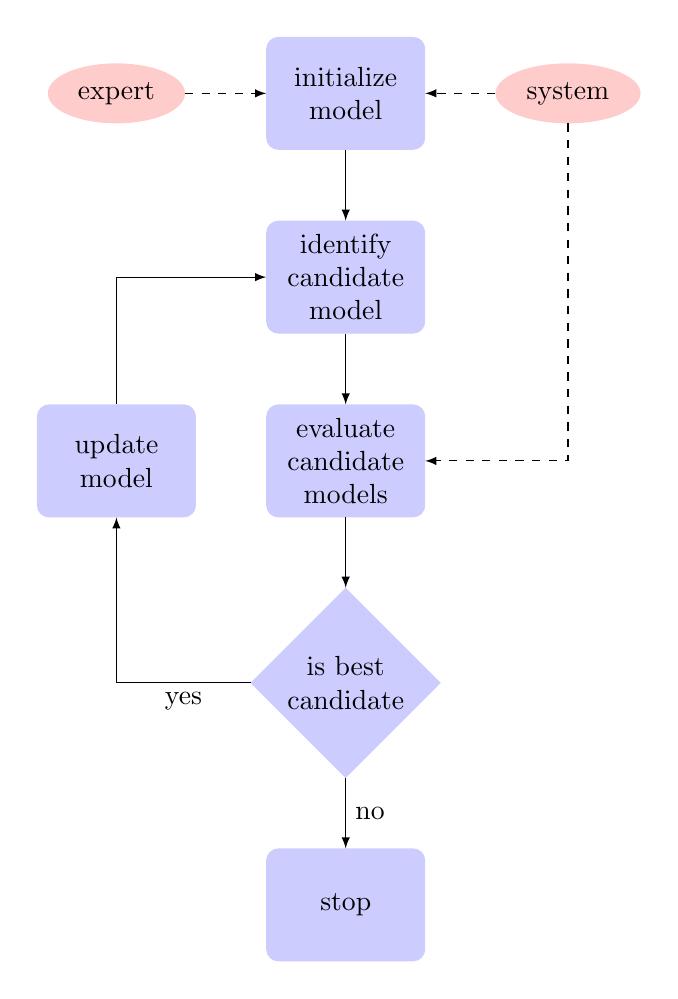
\begin{tikzpicture}[auto]
\tikzstyle{decision} = [diamond, draw=blue!20, thick, fill=blue!20,
text width=4.5em, text badly centered, inner sep=1pt]
\tikzstyle{block} = [rectangle, draw=blue!20, thick, fill=blue!20,
text width=5em, text centered, rounded corners, minimum height=4em]
\tikzstyle{line} = [draw, thick, -latex’,shorten >=2pt];
\tikzstyle{cloud} = [draw=red!20, thick, ellipse,fill=red!20, minimum height=2em];
\matrix [column sep=7mm,row sep=9mm]
{
% row 1
\node [cloud] (expert) {expert}; &
\node [block] (init) {initialize model}; &
\node [cloud] (system) {system}; \\
% row 2
& \node [block] (identify) {identify candidate model}; & \\
% row 3
\node [block] (update) {update model}; &
\node [block] (evaluate) {evaluate candidate models}; & \\
% row 4
& \node [decision] (decide) {is best candidate}; & \\
% row 5
& \node [block] (stop) {stop}; & \\
};
%\tikzstyle{every path}=[line]
\draw[->,>=latex] (init) -- (identify);
\draw[->,>=latex] (identify) -- (evaluate);
\draw[->,>=latex] (evaluate) -- (decide);
\draw[->,>=latex] (update) |- (identify);
\draw[->,>=latex] (decide) -| node [near start] {yes} (update);
\draw[->,>=latex] (decide) -- node [midway] {no} (stop);
\draw[->,>=latex] [dashed] (expert) -- (init);
\draw[->,>=latex] [dashed] (system) -- (init);
\draw[->,>=latex] [dashed] (system) |- (evaluate);
\end{tikzpicture}









\newpage

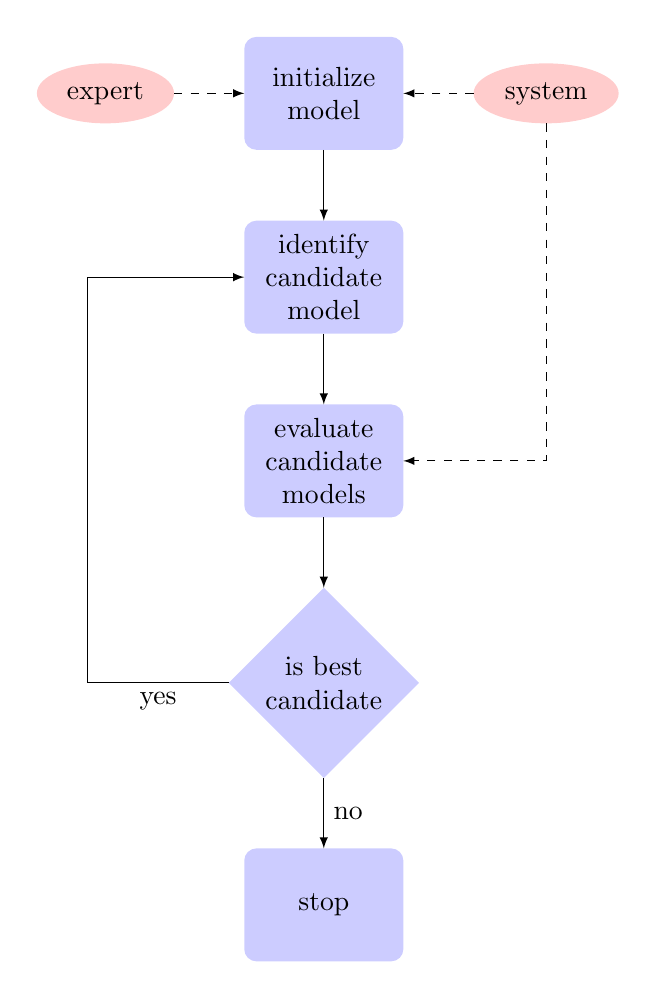
\begin{tikzpicture}[auto]
\tikzstyle{decision} = [diamond, draw=blue!20, thick, fill=blue!20,
text width=4.5em, text badly centered, inner sep=1pt]
\tikzstyle{block} = [rectangle, draw=blue!20, thick, fill=blue!20,
text width=5em, text centered, rounded corners, minimum height=4em]
\tikzstyle{line} = [draw, thick, -latex’,shorten >=2pt];
\tikzstyle{cloud} = [draw=red!20, thick, ellipse,fill=red!20, minimum height=2em];
\matrix [column sep=7mm,row sep=9mm]
{
% row 1
\node [cloud] (expert) {expert}; &
\node [block] (init) {initialize model}; &
\node [cloud] (system) {system}; \\
% row 2
& \node [block] (identify) {identify candidate model}; & \\
% row 3
\node  (update) {}; &
\node [block] (evaluate) {evaluate candidate models}; & \\
% row 4
& \node [decision] (decide) {is best candidate}; & \\
% row 5
& \node [block] (stop) {stop}; & \\
};
%\tikzstyle{every path}=[line]
\draw[->,>=latex] (init) -- (identify);
\draw[->,>=latex] (identify) -- (evaluate);
\draw[->,>=latex] (evaluate) -- (decide);
%\draw[->,>=latex] (update) |- (identify);
\draw[->,>=latex] (decide) -| node [near start] {yes} ($(decide)+(-3,3)$) |- (identify);
\draw[->,>=latex] (decide) -- node [midway] {no} (stop);
\draw[->,>=latex] [dashed] (expert) -- (init);
\draw[->,>=latex] [dashed] (system) -- (init);
\draw[->,>=latex] [dashed] (system) |- (evaluate);
\end{tikzpicture}












\newpage

\begin{tikzpicture}[auto]
\tikzstyle{decision} = [diamond, draw=blue!20, thick, fill=blue!20,
text width=4.5em, text badly centered, inner sep=1pt]
\tikzstyle{block} = [rectangle, draw=blue!20, thick, fill=blue!20,
text width=5em, text centered, rounded corners, minimum height=4em]
\tikzstyle{line} = [draw, thick, -latex’,shorten >=2pt];
\tikzstyle{cloud} = [draw=red!20, thick, ellipse,fill=red!20, minimum height=2em];
\matrix [column sep=7mm,row sep=9mm]
{
% row 1
\node [cloud] (expert) {شروع}; &
\node [block] (init) {گرفتن ورودی  }; &
\node [cloud] (system) {سیستم}; \\
% row 2
& \node [block] (identify) {تشخیص دادن}; & \\
% row 3
\node  (update) {}; &
\node [block] (evaluate) {  ارزیابی}; & \\
% row 4
& \node [decision] (decide) {شرط  }; & \\
% row 5
& \node [block] (stop) {توقف}; & \\
};
%\tikzstyle{every path}=[line]
\draw[->,>=latex] (init) -- (identify);
\draw[->,>=latex] (identify) -- (evaluate);
\draw[->,>=latex] (evaluate) -- (decide);
%\draw[->,>=latex] (update) |- (identify);
\draw[->,>=latex] (decide) -| node [near start] {بله} ($(decide)+(-3,3)$) |- (identify);
\draw[->,>=latex] (decide) -- node [midway] {خیر} (stop);
\draw[->,>=latex] [dashed] (expert) -- (init);
\draw[->,>=latex] [dashed] (system) -- (init);
\draw[->,>=latex] [dashed] (system) |- (evaluate);
\end{tikzpicture}







\newpage

\begin{tikzpicture}[auto]
\tikzstyle{decision} = [diamond, draw=black!50, thick, fill=white!20, text width=4.5em, text badly centered, inner sep=1pt]
\tikzstyle{block} = [rectangle, draw=black!50, thick, fill=white!20, text width=5em, text centered, rounded corners, minimum height=4em]
\tikzstyle{line} = [draw, thick, -latex’,shorten >=2pt];
\tikzstyle{cloud} = [draw=black!50, thick, ellipse,fill=white!20, minimum height=2em];
\matrix [column sep=7mm,row sep=9mm]
{
% row 1
\node [cloud] (expert) {شروع}; &
\node [block] (init) {گرفتن ورودی  }; &
\node [cloud] (system) {سیستم}; \\
% row 2
& \node [block] (identify) {تشخیص دادن}; & \\
% row 3
\node  (update) {}; &
\node [block] (evaluate) {  ارزیابی}; & \\
% row 4
& \node [decision] (decide) {شرط  }; & \\
% row 5
& \node [block] (stop) {توقف}; & \\
};
%\tikzstyle{every path}=[line]
\draw[->,>=latex] (init) -- (identify);
\draw[->,>=latex] (identify) -- (evaluate);
\draw[->,>=latex] (evaluate) -- (decide);
%\draw[->,>=latex] (update) |- (identify);
\draw[->,>=latex] (decide) -| node [near start] {بله} ($(decide)+(-3,3)$) |- (identify);
\draw[->,>=latex] (decide) -- node [midway] {خیر} (stop);
\draw[->,>=latex] [dashed] (expert) -- (init);
\draw[->,>=latex] [dashed] (system) -- (init);
\draw[->,>=latex] [dashed] (system) |- (evaluate);
\end{tikzpicture}









\newpage


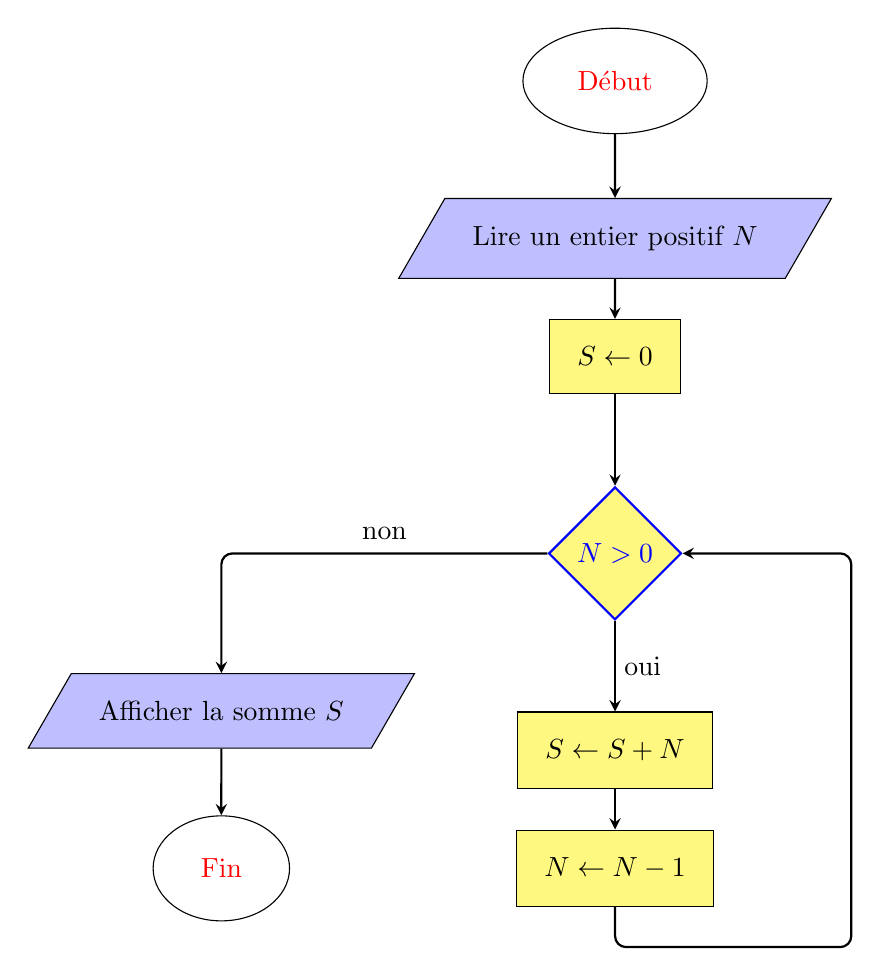
\begin{tikzpicture}
\tikzstyle{input}=[
        draw,
        trapezium,
        trapezium left angle=60,
        trapezium right angle=120,
        inner sep=10pt,
        fill=blue!25
]
\tikzstyle{output}=[
        draw,
        trapezium,
        trapezium left angle=60,
        trapezium right angle=120,
        inner sep=10pt,
        fill=blue!25
]
\tikzstyle{debutfin}=[ellipse,draw,text=red,inner sep=10pt]
\tikzstyle{instruct}=[rectangle,draw,fill=yellow!50,inner sep=10pt]
\tikzstyle{test}=[diamond, aspect=1,thick,
draw=blue,fill=yellow!50,text=blue]
\tikzstyle{es}=[rectangle,draw,rounded corners=4pt,fill=blue!25,inner sep=10pt]
%styledesflèches
\tikzstyle{suite}=[->,>=stealth,thick,rounded corners=4pt]
%placementdesnœuds
\node[debutfin] (debut) at (0,6) {Début};
\node[input] (lire) at (0,4) {Lire un entier positif $N$};
\node[instruct] (init) at (0,2.5) {$S\leftarrow 0$};
\node[test] (test) at (0,0) {$N>0$};
\node[instruct] (plus) at (0,-2.5) {$S\leftarrow S+N$};
\node[instruct] (moins) at (0,-4) {$N\leftarrow N-1$};
\node[output] (afficher) at (-5,-2) {Afficher la somme $S$};
\node[debutfin] (fin) at (-5,-4) {Fin};
%Placementdesflèches
\draw[suite] (debut) -- (lire);
\draw[suite] (lire) -- (init);
\draw[suite] (init) -- (test.north);
\draw[suite] (test) -- (plus) node[midway,xshift=10pt]{oui};
\draw[suite] (plus) -- (moins);
\draw[suite] (moins) |- (3,-5) |- (test.east);
\draw[suite] (test) -| (afficher) node[near start,yshift=7pt]{non};
\draw[suite] (afficher) -- (fin);
\end{tikzpicture}










\newpage

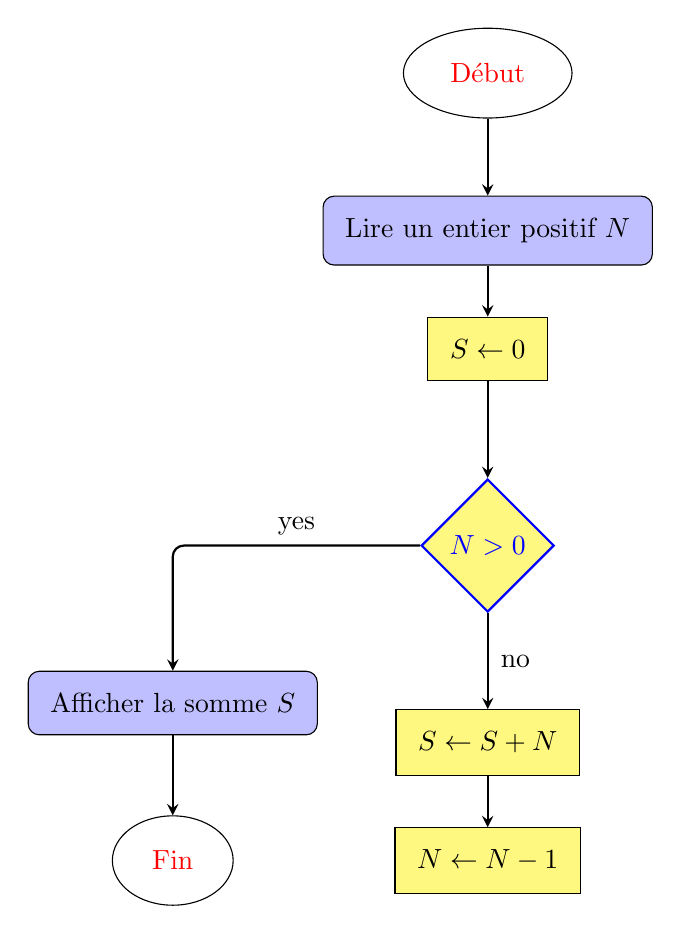
\begin{tikzpicture}
\tikzstyle{debutfin}=[ellipse,draw,text=red,inner sep=8pt]
\tikzstyle{instruct}=[rectangle,draw,fill=yellow!50,inner sep=8pt]
\tikzstyle{test}=[diamond, aspect=1,thick,
draw=blue,fill=yellow!50,text=blue]
\tikzstyle{es}=[rectangle,draw,rounded corners=4pt,fill=blue!25,inner sep=8pt]

\node[debutfin] (debut) at (0,6) {Début};
\node[es] (lire) at (0,4) {Lire un entier positif $N$};
\node[test] (test) at (0,0) {$N>0$};
\node[instruct] (init) at (0,2.5) {$S\leftarrow 0$};
\node[instruct] (plus) at (0,-2.5) {$S\leftarrow S+N$};
\node[instruct] (moins) at (0,-4) {$N\leftarrow N-1$};

\node[es] (afficher) at (-4,-2) {Afficher la somme $S$};
\node[debutfin] (fin) at (-4,-4) {Fin};

\tikzstyle{suite}=[->,>=stealth,thick,rounded corners=4pt]
\draw[suite] (debut) -- (lire);
\draw[suite] (lire) -- (init);
\draw[suite] (init) -- (test.north);
\draw[suite] (test) -- node[midway,xshift=10pt] {no} (plus);
\draw[suite] (plus) -- (moins);
\draw[suite] (test) -|  node[near start,yshift=7pt] {yes} (afficher);
\draw[suite] (afficher) -- (fin);

\end{tikzpicture}













\newpage


\begin{tikzpicture}
\tikzstyle{input}=[
        draw,
        trapezium,
        trapezium left angle=60,
        trapezium right angle=120,
        inner sep=10pt,
        fill=blue!25
]
\tikzstyle{output}=[
        draw,
        trapezium,
        trapezium left angle=60,
        trapezium right angle=120,
        inner sep=10pt,
        fill=blue!25
]
\tikzstyle{debutfin}=[ellipse,draw,text=red,inner sep=10pt]
\tikzstyle{instruct}=[rectangle,draw,fill=yellow!50,inner sep=10pt]
\tikzstyle{test}=[diamond, aspect=1,thick,
draw=blue,fill=yellow!50,text=blue]
\tikzstyle{es}=[rectangle,draw,rounded corners=4pt,fill=blue!25,inner sep=10pt]
%styledesflèches
\tikzstyle{suite}=[->,>=stealth,thick,rounded corners=4pt]
%placementdesnœuds
\node[debutfin] (debut) at (0,6) {شروع};
\node[input] (lire) at (0,4) {گرفتن ورودی};
\node[instruct] (init) at (0,2.5) {$S\leftarrow 0$};
\node[test] (test) at (0,0) {$N>0$};
\node[instruct] (plus) at (0,-2.5) {$S\leftarrow S+N$};
\node[instruct] (moins) at (0,-4) {$N\leftarrow N-1$};
\node[output] (afficher) at (-5,-2) {چاپ در خروجی};
\node[debutfin] (fin) at (-5,-4) {پایان};
%Placementdesflèches
\draw[suite] (debut) -- (lire);
\draw[suite] (lire) -- (init);
\draw[suite] (init) -- (test.north);
\draw[suite] (test) -- (plus) node[midway,xshift=10pt]{بله};
\draw[suite] (plus) -- (moins);
\draw[suite] (moins) |- (3,-5) |- (test.east);
\draw[suite] (test) -| (afficher) node[near start,yshift=7pt]{خیر};
\draw[suite] (afficher) -- (fin);
\end{tikzpicture}












\newpage


\begin{tikzpicture}
\tikzstyle{input}=[
        draw,
        trapezium,
        trapezium left angle=60,
        trapezium right angle=120,
        inner sep=10pt,
        fill=white!25
]
\tikzstyle{output}=[
        draw,
        trapezium,
        trapezium left angle=60,
        trapezium right angle=120,
        inner sep=10pt,
        fill=white!25
]
\tikzstyle{debutfin}=[ellipse,draw,text=black,inner sep=10pt]
\tikzstyle{instruct}=[rectangle,draw,fill=white!50,inner sep=10pt]
\tikzstyle{test}=[diamond, aspect=1,thick,
draw=black,fill=white!50,text=black]
\tikzstyle{es}=[rectangle,draw,rounded corners=4pt,fill=white!25,inner sep=10pt]
%styledesflèches
\tikzstyle{suite}=[->,>=stealth,thick,rounded corners=4pt]
%placementdesnœuds
\node[debutfin] (debut) at (0,6) {شروع};
\node[input] (lire) at (0,4) {گرفتن ورودی};
\node[instruct] (init) at (0,2.5) {$S\leftarrow 0$};
\node[test] (test) at (0,0) {$N>0$};
\node[instruct] (plus) at (0,-2.5) {$S\leftarrow S+N$};
\node[instruct] (moins) at (0,-4) {$N\leftarrow N-1$};
\node[output] (afficher) at (-5,-2) {چاپ در خروجی};
\node[debutfin] (fin) at (-5,-4) {پایان};
%Placementdesflèches
\draw[suite] (debut) -- (lire);
\draw[suite] (lire) -- (init);
\draw[suite] (init) -- (test.north);
\draw[suite] (test) -- (plus) node[midway,xshift=10pt]{بله};
\draw[suite] (plus) -- (moins);
\draw[suite] (moins) |- (3,-5) |- (test.east);
\draw[suite] (test) -| (afficher) node[near start,yshift=7pt]{خیر};
\draw[suite] (afficher) -- (fin);
\end{tikzpicture}




\end{document}